\section{Computing error in specific observables}
\label{sec:specific}

\subsection{Basics}
We frequently perform molecular simulations to make quantitative estimates of quantities like pressure, free energy or yield strain.  When reporting these estimates, it is important to also provide an estimate of the uncertainty of the result, typically as a standard error.  The standard error is the standard deviation of the distribution of the results that would be obtained by repeating the simulation.  Several techniques to estimate the uncertainty are described below with varying levels of complexity and robustness.  Ultimately, a technique is robust if it can produce an uncertainty estimate that is consistent with the standard deviation of results from actually repeating the simulation and analysis of the data.  The standard deviation of results from independent results can also be used when other approaches fail.  When computing the uncertainty with this approach, it is important to ensure that each starting configuration is also independent.  The means to obtain independent starting configurations is system-dependent, but might involve repeating the protocol used to construct a configuration (solvating a protein, inserting liquid molecules in a box, etc.), using a new random seed.

\begin{table}
    \begin{tabular}{S S}
      \toprule
       {Pressure (MPa)} & {Density (mol/L)} \\
      0.001 & 3.007(3)e-4 \\
      0.010 & 0.003011(2) \\
      0.100 & 0.03039(16) \\
      1.000 & 52.1(5) \\
      \bottomrule
    \end{tabular}
  \caption{Density as a function of pressure for water at a temperature of 400K}
  \label{tab:uncertainties}
\end{table}

When reporting quantities with uncertainties, only the digits that are significant should be included and the standard error should be placed after the value in parenthesis as the uncertainty in the last digit.  In general only one digit of uncertainty need be reported unless the digit is 1, in which case, it is helpful to report two digits (in order to avoid up to 50\% roundoff error in the uncertainty).  See the \TABLE{uncertainties} for examples from hypothetical isobaric simulations of water.

\subsection{Assessing quality of data}
%    - Data filtering [Paul]
Generally speaking, analysis routines that extract derived quantities from raw data are often formulated on the basis of physical intuition about how that data should behave.  Before proceeding to data analysis, it is therefore useful to assess the extent to which raw data conforms to these expectations and the requirements imposed by the analysis routines.  Such tasks help reduce subjectivity of predictions and offer insight into when a simulation protocol should be revisited to better understand their meaningfulness \cite{patrone1}.  Unfortunately, general recipes for assessing data quality are impossible to formulate, owing to the range of physical quantities of interest to modelers.  Nonetheless, a short example will help clarify the matter.

In the context of materials science, understanding when a structural material fails is critical for many engineering applications.  In the past decade, scientists have increasingly focused on modeling the yield-strain $\epsilon_y$, which is (loosely speaking) the amount of stretching (or strain) at which it deforms irreversibly.  Intuition and experiments tells us that upon deforming a material by a fraction $1+\epsilon$, it should recover its original dimensions if $\epsilon \le \epsilon_y$ and have a residual strain $\epsilon_r = \epsilon - \epsilon_y$ if $\epsilon \ge \epsilon_y$ \cite{patrone2}.  Owing to the time-scale limitations of MD, it is also reasonable to expect that the transition in $\epsilon_r$ around yield will be smooth and not piecewise linear.  Thus, if we fit residual strain to a hyperbola, the proximity of data to the asymptotes illustrates the extent to which simulated $\epsilon_r$ conforms to the expectation that $\epsilon_r=0$ when $\epsilon < \epsilon_y$.  See Fig.~\ref{fig:yield}.

\begin{figure}
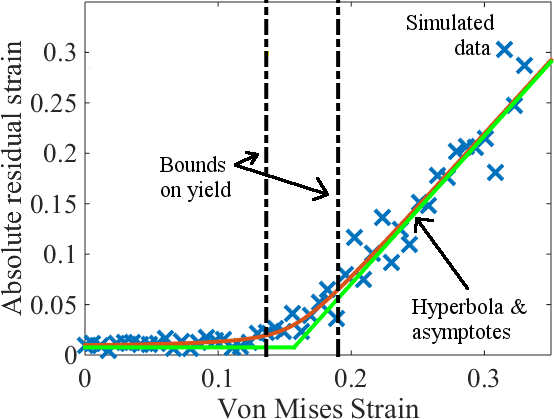
\includegraphics[width=8cm]{hyperbola.png}\caption{Yield strain tn $\epsilon_r$ as a function of applied strain $\epsilon$.  Blue $\times$ denote simulated data, whereas the smooth curve is a hyperbola fit to the data.  The green lines are asymptotes; their intersection can be taken as an estimate of $\epsilon_y$.    Bounds on yield are computed by the synthetic data method discussed in the next section.}\label{fig:yield}
\end{figure}

\subsection{Block averaging}

The uncertainty of a simulation obsverable can be estimated from the fluctuations in the quantity along with the fact that (in the absence of correlation) the squared uncertainty will be inversely proportional to the number of samples.  Block averages can be used instead of individual samples to avoid correlation in the samples while using all the data so long as the block averages are large enough to be uncorrelated \cite{Friedberg1970,FrenkelSmit2002}.  The uncertainty is expressed as
\begin{equation}
  \sigma = \sigma_{\rm blocks}/M^{1/2}
\end{equation}
where $\sigma_{\rm blocks}$ is the standard deviation of the block averages and $M$ is the number of blocks.

Since the approach assumes that the blocks are uncorrelated, it is important to check for correlation and try to eliminate it (by using longer blocks) or account for it.  One approach is to consider the uncertainty computed with blocks of increasing size and look for a plateau.  Another approach is to measure the block correlation and to use it to improve the uncertainty estimate \cite{Kolafa1986}.

\subsection{Propagation of uncertainty}

The quantities we are most interested in may not be simulation observables.  For instance, the free energy difference between two states might be measured by free energy perturbation, expressed as a function of the average of another quantity \cite{Taylor1997}.
\begin{equation}
\beta \Delta A = -\ln \left< \exp \left(-\beta \Delta U\right) \right>
\end{equation}
Although $\exp(-\beta \Delta U)$ can be measured during the simulation and its uncertainty can be estimated directly using block averages as described above, $\beta \Delta A$ cannot be handled the same way.  If we compute $\beta \Delta A$ for each block, the values will tend to take extremely positive whenever the perturbation does poorly (where $\Delta U$ is consistently large).  In the pathological case, $\Delta U$ might be $\infty$ for every sample in a block and the $\beta \Delta A=-\ln 0$ cannot be computed. Instead of using block averages for $\beta \Delta A$, its uncertainty can be expressed as a first-order Taylor series expansion
\begin{equation}
  \sigma_{\beta \Delta A} = \sigma_{\exp(\beta \Delta U)} / \left< \exp \left(-\beta \Delta U\right) \right>
  \label{eq:propagation_bDA}
\end{equation}

Propagation of uncertainty is needed whenever the derived quantity can be expressed only as a function of other averages.  It might also be needed when the derived quantity is of a function of quantities measured in separate simulations, such as $<U(T_2)>-<U(T_1)>$.  If a derived quantity is a function of multiple observables measured within a single simulation, then terms must be included to account for the correlation between those observables.

The Taylor series approach works well in most cases and easy to use, but does have limitations.  Because this approach is based on a first-order Taylor series, propagation of uncertainty can fail in cases where a non-linear formula is used and the uncertainty is very large or the distribution of input averages is not Gaussian.  For instance, the uncertainty in $\beta \Delta A$ as prescribed by Eq.~\ref{eq:propagation_bDA} cannot exceed unity no matter how short the simulation is or how bad the sampling is.  If there is doubt as to the quality of the computed uncertainty, the uncertainty can be computed with alternative approaches such as bootstrapping to verify the Taylor series results or to identify an alternative approach that works better.

\subsection{Bootstrapping}

The Taylor series approach may fail in some situations, either because a derived quantity cannot be expressed as a function of the measured simulation data or because the first-order truncation of the series is too severe.  Bootstrapping may still be able to yield an uncertainty for these more complicated cases because it does not need to understand the nature of the relationship between the derived quantity and the simulation observables \cite{Tibshirani1998}.  In nonparametric bootsrapping, new, ``synthetic'' data sets (corresponding to hypothetical simulation runs) are created by drawing samples from the original collection that was generated during the actual run.  The same sample may be selected twice, while others may not be selected at all (thus, this is sometimes called the replacement method).  In doing so, these synthetic sets will be different even though they all have the same number of samples and draw from the same pool of data.  Having created a new set, the data is analyzed to determine the derived quantity of interest.  This process is repeated to produce multiple estimates of the quantity; the uncertainty is the standard deviation of the computed quantities from the generated sets. Because the process uses original simulation samples, it does not need to make assumptions about the distribution of samples and works well even when the Taylor series approach fails.

The process described above assumes that the original simulation data is uncorrelated.  If this is not the case, then the resampling method can be reformulated in one of two ways.  The first option is to estimate the number of independent samples in the original set and to pull only that many samples to create the new data sets.  The second option is to group the samples into blocks that are uncorrelated and to then use the block averages as the samples for bootstrapping.  

An alternate approach that can directly account for correlations is called parametric bootstrapping.  The main idea behind this method is to model the original data as a deterministic function (which can be zero, constant, or have free parameters) plus additive noise.  The parameters of this model, including the structure of the noise (i.e.\ its covariance), can be determined through a statistical inference procedure.  Having calibrated the model, random number generators can be used to sample the noise, which is then added back to the trial function to generate a synthetic data set.   As with the nonparametric bootstrap, the generated data can be used to compute the derived quantity of interest, and the uncertainty can be obtained from the statistics of the values compute with different generated sets.

To further clarify the procedure of parametric boostrapping, consider the simplest case in which the data is a collection of uncorrelated random variables fluctuating about a constant mean.  In this situation, one could estimate (I) the deterministic part of a parametric model using the sample mean $\mu$ of the data, and (II) the stochastic part as a Gaussian random variable whose variance equals the sample variance.  If instead the data are correlated (e.g.\ as in a time-series of simulated observables),  one can postulate a covariance function to describe the structure of this randomness.  Often these covariance functions are formulated with free parameters (often called ``hyperparameters'') that characterize properties such as the noise-scale and characteristic length of correlations \cite{Rasmussen}.  In such cases, determining the hyperparameters may require more sophisticated techinques such as maximum likelihood analyses or Bayesian approaches; see, for example, Ref.~\cite{Rasmussen}.  See also Refs.~\cite{patrone1,patrone2,patrone3,patrone4} for examples and practical implementations applied to cases in which the determinsitic component of the data is not constant.  


\subsection{Dark uncertainty analyses}
%- ‘Dark uncertainty’ analysis [Paul]

In some cases, multiple simulations of the same physical observable $\tau$ may yield predictions whose error bars do not overlap.  This situation can arise, for example, in simulations of the glass transition temperature when undersampling the crosslinked network structure of certain polymers.  In such cases, it is reasonable to postulate an unaccounted for source of uncertainty, which we colorfully refer to as ``dark uncertainty.''  In the context of a statistical model, we postulate that the probability of a simulation output depends on the unobserved or ``true'' mean value $\bar \tau$, an uncertainty $\sigma_i^2$ whose value is specific to the simulation (estimated, e.g.\ according to uncertainty propagation), and the unaccounted-for dark uncertinty $y^2$.  (For simplicity, the $\sigma_i^2$ and $y^2$ should be treated as variances.)  

While details are beyond this scope of this document, such a model motivates an estimate of $\bar \tau$ of the form 
\begin{align}
\bar \tau \approx \mathcal T \propto \sum_i \frac{T_i}{\sigma_i^2 + y^2}, \label{eq:darkmean}
\end{align}
where $T_i$ is the prediction from the $i$th simulation, $\sigma_i^2$ is its associated ``within-simulation'' uncertainty, and $y^2$ is the dark or between-simulation uncertainty; note that the latter does not depend on $i$.  The variable $y^2$ can be estimated from a maximum-likelihood analysis of the data and amounts to numerically solving a relatively simple nonlinear equation (see Ref.~\cite{patrone1}).  Equation~\eqref{eq:darkmean} is useful insofar as it weights simulated results according to their certainty while reducing the impact of overconfident predictions (e.g. having small $\sigma_i^2$).  Additional details on this method are provided in Ref.~\cite{patrone1} and the references contained therein.



- Basics: how to report, what goal to shoot for, significant figures
- When should you not trust uncertainties
    - Unknown unknowns
- If calculating a derived quantity, consider error in conversion from raw data 
    - Propagation of error (this doesn’t mean publishing your results!)
    - Taylor series expansion can handle cases where derived quantity is a direct function of measured data
    - Wikipedia: Propagation of uncertainty
    - Bootstrapping [Andrew/Dan S]
used for cases where the derived quantity is not simple function of the measured data.
An Introduction to the Bootstrap
    - Need to know correlation to correctly estimate sample size
    - Otherwise just gives relative uncertainty
- Correlation time analysis [Dan Z]
- Block averaging [Dan Z/Alan?/Dan S] Flyvjberg and Petersen 
- MOST OF THESE ALGORITHMS FAIL IF THE TRAJECTORY IS WAY TOO SHORT
    - If you miss the timescale by enough, you can’t tell
    - YOU HAVE TO THINK ABOUT THIS IN ADVANCE
- Link out to transport doc
